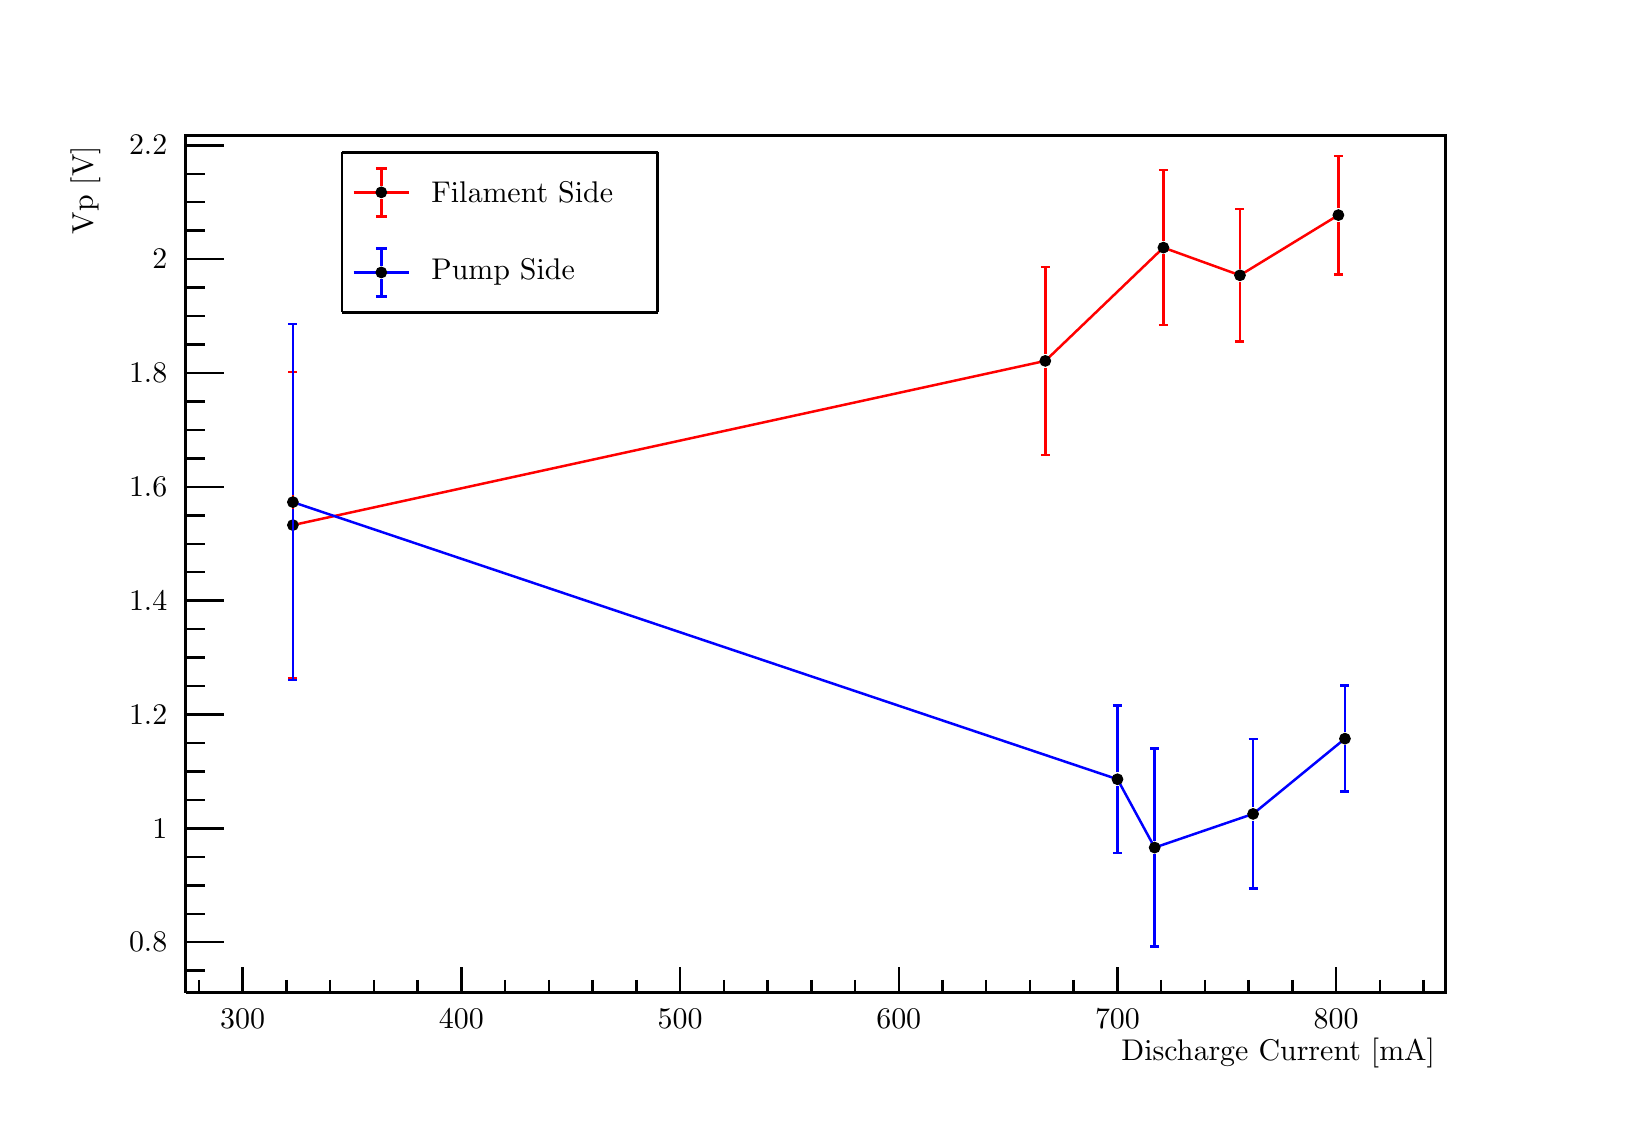
\begin{tikzpicture}
\pgfdeclareplotmark{cross} {
\pgfpathmoveto{\pgfpoint{-0.3\pgfplotmarksize}{\pgfplotmarksize}}
\pgfpathlineto{\pgfpoint{+0.3\pgfplotmarksize}{\pgfplotmarksize}}
\pgfpathlineto{\pgfpoint{+0.3\pgfplotmarksize}{0.3\pgfplotmarksize}}
\pgfpathlineto{\pgfpoint{+1\pgfplotmarksize}{0.3\pgfplotmarksize}}
\pgfpathlineto{\pgfpoint{+1\pgfplotmarksize}{-0.3\pgfplotmarksize}}
\pgfpathlineto{\pgfpoint{+0.3\pgfplotmarksize}{-0.3\pgfplotmarksize}}
\pgfpathlineto{\pgfpoint{+0.3\pgfplotmarksize}{-1.\pgfplotmarksize}}
\pgfpathlineto{\pgfpoint{-0.3\pgfplotmarksize}{-1.\pgfplotmarksize}}
\pgfpathlineto{\pgfpoint{-0.3\pgfplotmarksize}{-0.3\pgfplotmarksize}}
\pgfpathlineto{\pgfpoint{-1.\pgfplotmarksize}{-0.3\pgfplotmarksize}}
\pgfpathlineto{\pgfpoint{-1.\pgfplotmarksize}{0.3\pgfplotmarksize}}
\pgfpathlineto{\pgfpoint{-0.3\pgfplotmarksize}{0.3\pgfplotmarksize}}
\pgfpathclose
\pgfusepathqstroke
}
\pgfdeclareplotmark{cross*} {
\pgfpathmoveto{\pgfpoint{-0.3\pgfplotmarksize}{\pgfplotmarksize}}
\pgfpathlineto{\pgfpoint{+0.3\pgfplotmarksize}{\pgfplotmarksize}}
\pgfpathlineto{\pgfpoint{+0.3\pgfplotmarksize}{0.3\pgfplotmarksize}}
\pgfpathlineto{\pgfpoint{+1\pgfplotmarksize}{0.3\pgfplotmarksize}}
\pgfpathlineto{\pgfpoint{+1\pgfplotmarksize}{-0.3\pgfplotmarksize}}
\pgfpathlineto{\pgfpoint{+0.3\pgfplotmarksize}{-0.3\pgfplotmarksize}}
\pgfpathlineto{\pgfpoint{+0.3\pgfplotmarksize}{-1.\pgfplotmarksize}}
\pgfpathlineto{\pgfpoint{-0.3\pgfplotmarksize}{-1.\pgfplotmarksize}}
\pgfpathlineto{\pgfpoint{-0.3\pgfplotmarksize}{-0.3\pgfplotmarksize}}
\pgfpathlineto{\pgfpoint{-1.\pgfplotmarksize}{-0.3\pgfplotmarksize}}
\pgfpathlineto{\pgfpoint{-1.\pgfplotmarksize}{0.3\pgfplotmarksize}}
\pgfpathlineto{\pgfpoint{-0.3\pgfplotmarksize}{0.3\pgfplotmarksize}}
\pgfpathclose
\pgfusepathqfillstroke
}
\pgfdeclareplotmark{newstar} {
\pgfpathmoveto{\pgfqpoint{0pt}{\pgfplotmarksize}}
\pgfpathlineto{\pgfqpointpolar{44}{0.5\pgfplotmarksize}}
\pgfpathlineto{\pgfqpointpolar{18}{\pgfplotmarksize}}
\pgfpathlineto{\pgfqpointpolar{-20}{0.5\pgfplotmarksize}}
\pgfpathlineto{\pgfqpointpolar{-54}{\pgfplotmarksize}}
\pgfpathlineto{\pgfqpointpolar{-90}{0.5\pgfplotmarksize}}
\pgfpathlineto{\pgfqpointpolar{234}{\pgfplotmarksize}}
\pgfpathlineto{\pgfqpointpolar{198}{0.5\pgfplotmarksize}}
\pgfpathlineto{\pgfqpointpolar{162}{\pgfplotmarksize}}
\pgfpathlineto{\pgfqpointpolar{134}{0.5\pgfplotmarksize}}
\pgfpathclose
\pgfusepathqstroke
}
\pgfdeclareplotmark{newstar*} {
\pgfpathmoveto{\pgfqpoint{0pt}{\pgfplotmarksize}}
\pgfpathlineto{\pgfqpointpolar{44}{0.5\pgfplotmarksize}}
\pgfpathlineto{\pgfqpointpolar{18}{\pgfplotmarksize}}
\pgfpathlineto{\pgfqpointpolar{-20}{0.5\pgfplotmarksize}}
\pgfpathlineto{\pgfqpointpolar{-54}{\pgfplotmarksize}}
\pgfpathlineto{\pgfqpointpolar{-90}{0.5\pgfplotmarksize}}
\pgfpathlineto{\pgfqpointpolar{234}{\pgfplotmarksize}}
\pgfpathlineto{\pgfqpointpolar{198}{0.5\pgfplotmarksize}}
\pgfpathlineto{\pgfqpointpolar{162}{\pgfplotmarksize}}
\pgfpathlineto{\pgfqpointpolar{134}{0.5\pgfplotmarksize}}
\pgfpathclose
\pgfusepathqfillstroke
}
\definecolor{c}{rgb}{1,1,1};
\draw [color=c, fill=c] (0,0) rectangle (20,13.6103);
\draw [color=c, fill=c] (2,1.36103) rectangle (18,12.2493);
\definecolor{c}{rgb}{0,0,0};
\draw [c,line width=0.9] (2,1.36103) -- (2,12.2493) -- (18,12.2493) -- (18,1.36103) -- (2,1.36103);
\definecolor{c}{rgb}{1,1,1};
\draw [color=c, fill=c] (2,1.36103) rectangle (18,12.2493);
\definecolor{c}{rgb}{0,0,0};
\draw [c,line width=0.9] (2,1.36103) -- (2,12.2493) -- (18,12.2493) -- (18,1.36103) -- (2,1.36103);
\draw [c,line width=0.9] (2,1.36103) -- (18,1.36103);
\draw [c,line width=0.9] (2.72222,1.68768) -- (2.72222,1.36103);
\draw [c,line width=0.9] (3.27778,1.52436) -- (3.27778,1.36103);
\draw [c,line width=0.9] (3.83333,1.52436) -- (3.83333,1.36103);
\draw [c,line width=0.9] (4.38889,1.52436) -- (4.38889,1.36103);
\draw [c,line width=0.9] (4.94444,1.52436) -- (4.94444,1.36103);
\draw [c,line width=0.9] (5.5,1.68768) -- (5.5,1.36103);
\draw [c,line width=0.9] (6.05556,1.52436) -- (6.05556,1.36103);
\draw [c,line width=0.9] (6.61111,1.52436) -- (6.61111,1.36103);
\draw [c,line width=0.9] (7.16667,1.52436) -- (7.16667,1.36103);
\draw [c,line width=0.9] (7.72222,1.52436) -- (7.72222,1.36103);
\draw [c,line width=0.9] (8.27778,1.68768) -- (8.27778,1.36103);
\draw [c,line width=0.9] (8.83333,1.52436) -- (8.83333,1.36103);
\draw [c,line width=0.9] (9.38889,1.52436) -- (9.38889,1.36103);
\draw [c,line width=0.9] (9.94444,1.52436) -- (9.94444,1.36103);
\draw [c,line width=0.9] (10.5,1.52436) -- (10.5,1.36103);
\draw [c,line width=0.9] (11.0556,1.68768) -- (11.0556,1.36103);
\draw [c,line width=0.9] (11.6111,1.52436) -- (11.6111,1.36103);
\draw [c,line width=0.9] (12.1667,1.52436) -- (12.1667,1.36103);
\draw [c,line width=0.9] (12.7222,1.52436) -- (12.7222,1.36103);
\draw [c,line width=0.9] (13.2778,1.52436) -- (13.2778,1.36103);
\draw [c,line width=0.9] (13.8333,1.68768) -- (13.8333,1.36103);
\draw [c,line width=0.9] (14.3889,1.52436) -- (14.3889,1.36103);
\draw [c,line width=0.9] (14.9444,1.52436) -- (14.9444,1.36103);
\draw [c,line width=0.9] (15.5,1.52436) -- (15.5,1.36103);
\draw [c,line width=0.9] (16.0556,1.52436) -- (16.0556,1.36103);
\draw [c,line width=0.9] (16.6111,1.68768) -- (16.6111,1.36103);
\draw [c,line width=0.9] (2.72222,1.68768) -- (2.72222,1.36103);
\draw [c,line width=0.9] (2.16667,1.52436) -- (2.16667,1.36103);
\draw [c,line width=0.9] (16.6111,1.68768) -- (16.6111,1.36103);
\draw [c,line width=0.9] (17.1667,1.52436) -- (17.1667,1.36103);
\draw [c,line width=0.9] (17.7222,1.52436) -- (17.7222,1.36103);
\draw [anchor=base] (2.72222,0.911891) node[scale=1.08185, color=c, rotate=0]{300};
\draw [anchor=base] (5.5,0.911891) node[scale=1.08185, color=c, rotate=0]{400};
\draw [anchor=base] (8.27778,0.911891) node[scale=1.08185, color=c, rotate=0]{500};
\draw [anchor=base] (11.0556,0.911891) node[scale=1.08185, color=c, rotate=0]{600};
\draw [anchor=base] (13.8333,0.911891) node[scale=1.08185, color=c, rotate=0]{700};
\draw [anchor=base] (16.6111,0.911891) node[scale=1.08185, color=c, rotate=0]{800};
\draw [anchor= east] (18,0.598854) node[scale=1.08185, color=c, rotate=0]{Discharge Current [mA]};
\draw [c,line width=0.9] (2,1.36103) -- (2,12.2493);
\draw [c,line width=0.9] (2.48,2.00249) -- (2,2.00249);
\draw [c,line width=0.9] (2.24,2.36394) -- (2,2.36394);
\draw [c,line width=0.9] (2.24,2.72539) -- (2,2.72539);
\draw [c,line width=0.9] (2.24,3.08684) -- (2,3.08684);
\draw [c,line width=0.9] (2.48,3.44828) -- (2,3.44828);
\draw [c,line width=0.9] (2.24,3.80973) -- (2,3.80973);
\draw [c,line width=0.9] (2.24,4.17118) -- (2,4.17118);
\draw [c,line width=0.9] (2.24,4.53263) -- (2,4.53263);
\draw [c,line width=0.9] (2.48,4.89407) -- (2,4.89407);
\draw [c,line width=0.9] (2.24,5.25552) -- (2,5.25552);
\draw [c,line width=0.9] (2.24,5.61697) -- (2,5.61697);
\draw [c,line width=0.9] (2.24,5.97842) -- (2,5.97842);
\draw [c,line width=0.9] (2.48,6.33986) -- (2,6.33986);
\draw [c,line width=0.9] (2.24,6.70131) -- (2,6.70131);
\draw [c,line width=0.9] (2.24,7.06276) -- (2,7.06276);
\draw [c,line width=0.9] (2.24,7.42421) -- (2,7.42421);
\draw [c,line width=0.9] (2.48,7.78566) -- (2,7.78566);
\draw [c,line width=0.9] (2.24,8.1471) -- (2,8.1471);
\draw [c,line width=0.9] (2.24,8.50855) -- (2,8.50855);
\draw [c,line width=0.9] (2.24,8.87) -- (2,8.87);
\draw [c,line width=0.9] (2.48,9.23145) -- (2,9.23145);
\draw [c,line width=0.9] (2.24,9.59289) -- (2,9.59289);
\draw [c,line width=0.9] (2.24,9.95434) -- (2,9.95434);
\draw [c,line width=0.9] (2.24,10.3158) -- (2,10.3158);
\draw [c,line width=0.9] (2.48,10.6772) -- (2,10.6772);
\draw [c,line width=0.9] (2.24,11.0387) -- (2,11.0387);
\draw [c,line width=0.9] (2.24,11.4001) -- (2,11.4001);
\draw [c,line width=0.9] (2.24,11.7616) -- (2,11.7616);
\draw [c,line width=0.9] (2.48,12.123) -- (2,12.123);
\draw [c,line width=0.9] (2.48,2.00249) -- (2,2.00249);
\draw [c,line width=0.9] (2.24,1.64104) -- (2,1.64104);
\draw [c,line width=0.9] (2.48,12.123) -- (2,12.123);
\draw [anchor= east] (1.9,2.00249) node[scale=1.08185, color=c, rotate=0]{0.8};
\draw [anchor= east] (1.9,3.44828) node[scale=1.08185, color=c, rotate=0]{1};
\draw [anchor= east] (1.9,4.89407) node[scale=1.08185, color=c, rotate=0]{1.2};
\draw [anchor= east] (1.9,6.33986) node[scale=1.08185, color=c, rotate=0]{1.4};
\draw [anchor= east] (1.9,7.78566) node[scale=1.08185, color=c, rotate=0]{1.6};
\draw [anchor= east] (1.9,9.23145) node[scale=1.08185, color=c, rotate=0]{1.8};
\draw [anchor= east] (1.9,10.6772) node[scale=1.08185, color=c, rotate=0]{2};
\draw [anchor= east] (1.9,12.123) node[scale=1.08185, color=c, rotate=0]{2.2};
\draw [anchor= east] (0.726934,12.2493) node[scale=1.08185, color=c, rotate=90]{Vp [V]};
\definecolor{c}{rgb}{1,0,0};
\draw [c,line width=0.9] (3.36111,7.30001) -- (12.9167,9.38528) -- (14.4167,10.8241) -- (15.3889,10.4724) -- (16.6389,11.237);
\definecolor{c}{rgb}{0,0,0};
\foreach \P in {(3.36111,7.30001), (12.9167,9.38528), (14.4167,10.8241), (15.3889,10.4724), (16.6389,11.237)}{\draw[mark options={color=c,fill=c},mark size=1.921922pt,mark=*] plot coordinates {\P};}
\definecolor{c}{rgb}{1,0,0};
\draw [c,line width=0.9] (3.36111,7.38597) -- (3.36111,9.24498);
\draw [c,line width=0.9] (3.3038,9.24498) -- (3.41842,9.24498);
\draw [c,line width=0.9] (3.36111,7.21405) -- (3.36111,5.35505);
\draw [c,line width=0.9] (3.3038,5.35505) -- (3.41842,5.35505);
\draw [c,line width=0.9] (12.9167,9.47124) -- (12.9167,10.5776);
\draw [c,line width=0.9] (12.8594,10.5776) -- (12.974,10.5776);
\draw [c,line width=0.9] (12.9167,9.29932) -- (12.9167,8.19297);
\draw [c,line width=0.9] (12.8594,8.19297) -- (12.974,8.19297);
\draw [c,line width=0.9] (14.4167,10.91) -- (14.4167,11.8082);
\draw [c,line width=0.9] (14.3594,11.8082) -- (14.474,11.8082);
\draw [c,line width=0.9] (14.4167,10.7381) -- (14.4167,9.83996);
\draw [c,line width=0.9] (14.3594,9.83996) -- (14.474,9.83996);
\draw [c,line width=0.9] (15.3889,10.5584) -- (15.3889,11.3133);
\draw [c,line width=0.9] (15.3316,11.3133) -- (15.4462,11.3133);
\draw [c,line width=0.9] (15.3889,10.3865) -- (15.3889,9.63154);
\draw [c,line width=0.9] (15.3316,9.63154) -- (15.4462,9.63154);
\draw [c,line width=0.9] (16.6389,11.323) -- (16.6389,11.9896);
\draw [c,line width=0.9] (16.5816,11.9896) -- (16.6962,11.9896);
\draw [c,line width=0.9] (16.6389,11.1511) -- (16.6389,10.4845);
\draw [c,line width=0.9] (16.5816,10.4845) -- (16.6962,10.4845);
\definecolor{c}{rgb}{0,0,1};
\draw [c,line width=0.9] (3.36111,7.67781) -- (3.36111,9.85224);
\draw [c,line width=0.9] (3.3038,9.85224) -- (3.41842,9.85224);
\draw [c,line width=0.9] (3.36111,7.50589) -- (3.36111,5.33145);
\draw [c,line width=0.9] (3.3038,5.33145) -- (3.41842,5.33145);
\draw [c,line width=0.9] (13.8333,4.15832) -- (13.8333,5.01127);
\draw [c,line width=0.9] (13.776,5.01127) -- (13.8906,5.01127);
\draw [c,line width=0.9] (13.8333,3.9864) -- (13.8333,3.13345);
\draw [c,line width=0.9] (13.776,3.13345) -- (13.8906,3.13345);
\draw [c,line width=0.9] (14.3056,3.2904) -- (14.3056,4.4604);
\draw [c,line width=0.9] (14.2482,4.4604) -- (14.3629,4.4604);
\draw [c,line width=0.9] (14.3056,3.11848) -- (14.3056,1.94847);
\draw [c,line width=0.9] (14.2482,1.94847) -- (14.3629,1.94847);
\draw [c,line width=0.9] (15.5556,3.718) -- (15.5556,4.58187);
\draw [c,line width=0.9] (15.4982,4.58187) -- (15.6129,4.58187);
\draw [c,line width=0.9] (15.5556,3.54608) -- (15.5556,2.68222);
\draw [c,line width=0.9] (15.4982,2.68222) -- (15.6129,2.68222);
\draw [c,line width=0.9] (16.7222,4.67367) -- (16.7222,5.26046);
\draw [c,line width=0.9] (16.6649,5.26046) -- (16.7795,5.26046);
\draw [c,line width=0.9] (16.7222,4.50175) -- (16.7222,3.91496);
\draw [c,line width=0.9] (16.6649,3.91496) -- (16.7795,3.91496);
\draw [c,line width=0.9] (3.36111,7.59185) -- (13.8333,4.07236) -- (14.3056,3.20444) -- (15.5556,3.63204) -- (16.7222,4.58771);
\definecolor{c}{rgb}{0,0,0};
\foreach \P in {(3.36111,7.59185), (13.8333,4.07236), (14.3056,3.20444), (15.5556,3.63204), (16.7222,4.58771)}{\draw[mark options={color=c,fill=c},mark size=1.921922pt,mark=*] plot coordinates {\P};}
\definecolor{c}{rgb}{1,1,1};
\draw [color=c, fill=c] (3.98281,10) rectangle (7.99427,12.0344);
\definecolor{c}{rgb}{0,0,0};
\draw [c,line width=0.9] (3.98281,10) -- (7.99427,10);
\draw [c,line width=0.9] (7.99427,10) -- (7.99427,12.0344);
\draw [c,line width=0.9] (7.99427,12.0344) -- (3.98281,12.0344);
\draw [c,line width=0.9] (3.98281,12.0344) -- (3.98281,10);
\draw [anchor= west] (4.98567,11.5258) node[scale=1.08185, color=c, rotate=0]{Filament Side};
\definecolor{c}{rgb}{1,0,0};
\draw [c,line width=0.9] (4.13324,11.5258) -- (4.83524,11.5258);
\draw [c,line width=0.9] (4.48424,11.6117) -- (4.48424,11.8309);
\draw [c,line width=0.9] (4.48424,11.4398) -- (4.48424,11.2206);
\draw [c,line width=0.9] (4.41404,11.8309) -- (4.55444,11.8309);
\draw [c,line width=0.9] (4.41404,11.2206) -- (4.55444,11.2206);
\definecolor{c}{rgb}{0,0,0};
\foreach \P in {(4.48424,11.5258)}{\draw[mark options={color=c,fill=c},mark size=1.921922pt,mark=*] plot coordinates {\P};}
\draw [anchor= west] (4.98567,10.5086) node[scale=1.08185, color=c, rotate=0]{Pump Side};
\definecolor{c}{rgb}{0,0,1};
\draw [c,line width=0.9] (4.13324,10.5086) -- (4.83524,10.5086);
\draw [c,line width=0.9] (4.48424,10.5946) -- (4.48424,10.8138);
\draw [c,line width=0.9] (4.48424,10.4226) -- (4.48424,10.2034);
\draw [c,line width=0.9] (4.41404,10.8138) -- (4.55444,10.8138);
\draw [c,line width=0.9] (4.41404,10.2034) -- (4.55444,10.2034);
\definecolor{c}{rgb}{0,0,0};
\foreach \P in {(4.48424,10.5086)}{\draw[mark options={color=c,fill=c},mark size=1.921922pt,mark=*] plot coordinates {\P};}
\end{tikzpicture}
